To effectively localize and navigate itself, the robot's algorithm first needs a map of its environment. This map consists of a probability grid with each square enclosing an area of \qty{5}{cm^2} in the real-world \parencite{hessRealtimeLoopClosure2016}. Since the map is formatted as a grayscale image file (PGM), the squares are referred to as pixels. Each pixel is assigned a value between 0 (white) and 1 (black), representing the probability of the pixel being occupied. A probability closer to 0 means the square is likely to be empty, while a probability closer to 1 means the square is likely to be occupied. An example map is shown in Figure \ref{fig:map}.

\begin{figure}[!htb]
    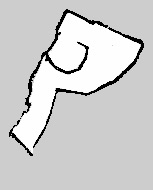
\includegraphics[width=4cm]{map.jpeg}
    \centering
    \caption{A grayscale map generated by a TurtleBot3.}
    \label{fig:map}
\end{figure}

\subsection{Building Submaps} \label{submaps}
The complete map of the environment is built by stitching multiple submaps together \parencite{hessRealtimeLoopClosure2016}. Each submap is built using a few consecutive LiDAR scans by aligning their coordinate frames. This project uses six scans per submap, but this parameter can be changed. The matrix transformation used to rotate counterclockwise and translate the scan on the XY-plane is given by
\[
    T_\xi p =
    \begin{bmatrix}
        \cos(\xi_\theta) & -\sin(\xi_\theta) \\
        \sin(\xi_\theta) & \cos(\xi_\theta)
    \end{bmatrix}p + \begin{bmatrix}
        \xi_x \\
        \xi_y
    \end{bmatrix},
\]
where $p$ is a hit point on the scan and $\xi=(\xi_x,\xi_y,\xi_\theta)$ is the scan's pose relative to the submap \parencite{RotationMatrix2024,hessRealtimeLoopClosure2016}. All the hit points in a single scan can be represented as $H=\{h_k\}_{k=1,\ldots,K},h_k\in\mathbb{R}^2$. In order to determine the pose of each scan, a scan matcher is used to ``[maximize] the probabilities at the scan points in the submap'' \parencite{hessRealtimeLoopClosure2016}. This ensures the best possible alignment and overlap between the scans in a submap. An optimizer, such as the Ceres Solver, is used to optimize the non-linear least squares problem
\[
    \argmin_{\xi} \sum_{k=1}^{K}(1 - M_\text{smooth}(T_\xi h_k))^2
\]
\parencite{SolvingNonlinearLeast,hessRealtimeLoopClosure2016}. Here, ``$T_\xi$ transforms [each hit point on a scan ($h_k$)] from the scan coordinate frame to the submap coordinate frame'' \parencite{hessRealtimeLoopClosure2016}. The $M_\text{smooth}$ function interpolates the discrete probabilities of each pixel in the submap into a continuous curve with bicubic interpolation, as shown in Figure \ref{fig:bicubic}. By plugging the transformed point into $M_\text{smooth}$, the current occupancy probability in the submap at that point is obtained. Thus, $1 - M_\text{smooth}(T_\xi h_k)$ represents the difference between the scan's probability and the submap's probability at that point. The square serves to amplify large differences and reduce small differences. By minimizing the sum of all these differences, the $\argmin$ function identifies the pose ($\xi$) that aligns the scan data most optimally with the existing submap, maximizing their overlap. Initially, this pose ($\xi$) can be estimated using the robot's odometry through dead reckoning.

\begin{figure}[!htb]
    \centering
    \subfloat[\centering Non-interpolated]{{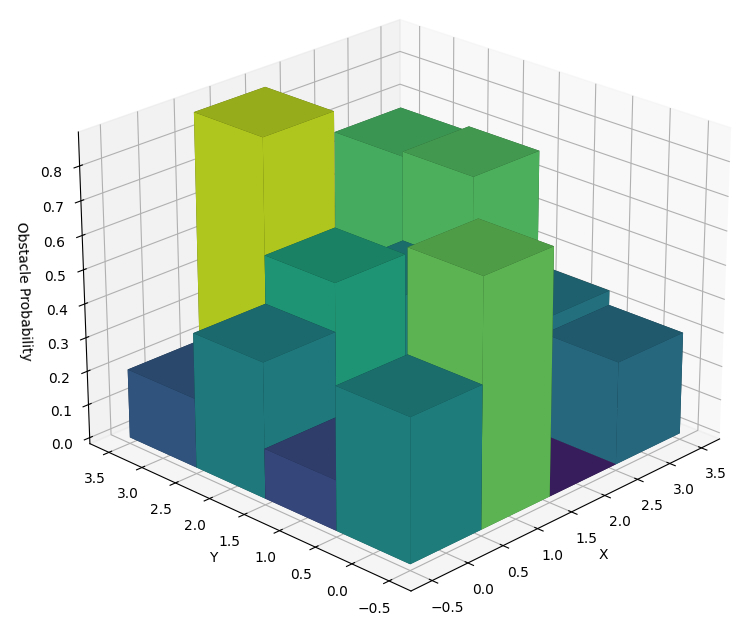
\includegraphics[width=5cm]{bicubic-ni} }}
    \qquad
    \subfloat[\centering Bicubic interpolation]{{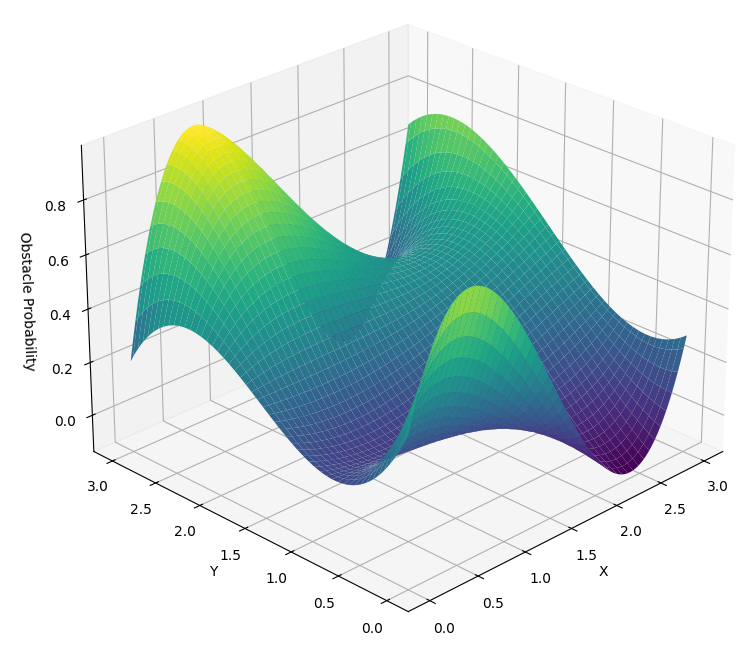
\includegraphics[width=5cm]{bicubic-bi} }}
    \caption{3D representation of the bicubic interpolation done by $M_\text{smooth}$ for a small submap.}
    \label{fig:bicubic}
\end{figure}

To insert a scan into a submap, each pixel that intersects a hit point is added to a ``hits'' list, and each pixel situated on the straight path from the robot's LiDAR sensor to a hit point, except for the ones also intersecting another hit point, is added to a ``misses'' list \parencite{hessRealtimeLoopClosure2016}. A probability value between 0 and 1 is then assigned to each pixel in both lists. If a pixel was never observed before in the submap, it is assigned a predefined probability of $p_{hit}$ or $p_{miss}$ depending on which list it is in. If a pixel was already observed, its old probability ($M_\text{old}$) can be updated by calculating a new probability ($M_\text{new}$) using the function
\[
    M_\text{new}(x)=clamp(odds^{-1}(odds(M_\text{old}(x))\cdot odds(p_\text{hit/miss}))),
\]
where $odds(p)=\frac{p}{1-p}$ and $odds^{-1}(p)=\frac{p}{1+p}$. The clamp function restricts probabilities to a predefined range to avoid issues with the $odds$ function and prevent the robot from treating cells with absolute certainty due to sensor errors. Given a scenario where $p_{hit}=0.750$ and a hit point intersects with an already observed pixel currently having a probability of 0.700, the new probability can be calculated as follows:
\begin{enumerate}
    \item $odds(p)=odds(0.75)=\frac{0.750}{1-0.750}=3.00$
    \item $odds(p)=odds(0.7)=\frac{0.700}{1-0.700}=2.33$
    \item $M_\text{new}(x)=clamp(odds^{-1}((2.33)(3.00)))=clamp(odds^{-1}(7.00))=\frac{7.00}{1+7.00}=0.875$
\end{enumerate}
Now, the probability of this pixel is changed to 0.875.

\subsection{Building a Map} \label{map}
By focusing solely on a few recent scans for submap creation, this method can slowly drift away from an accurate representation of the environment due to accumulated errors \parencite{hessRealtimeLoopClosure2016}. Hence, a second scan matcher runs to compare scans between submaps that overlap. When a match is identified, ``the... [estimated] relative pose [of the scan in its submap] is added to the optimization problem'' \parencite{hessRealtimeLoopClosure2016}. In other words, a constraint is added to stitch the submaps together. This loop closure optimization runs every few seconds to repair the accumulated error when the robot revisits a position. An optimizer, such as the Ceres Solver, can be used to solve the following non-linear least squares problem
\[
    \argmin_{\Xi^\text{m},\Xi^\text{s}} \frac{1}{2}\sum_{ij}\rho(E^2(\xi_i^\text{m},\xi_j^\text{s};\Sigma_{ij},\xi_{ij})),
\]
where $\Xi^\text{m}=\{\xi_i^\text{m}\}_{i=1,\ldots,m}$ are the submap poses, $\Xi^\text{s}=\{\xi_j^\text{s}\}_{j=1,\ldots,n}$ are the scan poses, and $\xi_{ij}$ is a relative pose constraint added by the second scan matcher \parencite{SolvingNonlinearLeast,hessRealtimeLoopClosure2016}. $\Sigma_{ij}$, which is estimated by the optimizer, is a covariance matrix associated with $\xi_{ij}$. A covariance matrix is a square matrix that describes the variance of individual variables (dispersion of data) and the covariance between pairs of variables (how the variables vary together) \parencite{CovarianceMatrixFormula}. In this case, it is used to estimate the uncertainty of $\xi_{ij}$. $\rho$ is a loss function used to minimize the impact of incorrect constraints added during the scan matching. The $E^2$ function is given by
\[
    E^2(\xi_i^\text{m},\xi_j^\text{s};\Sigma_{ij},\xi_{ij})=e(\xi_i^\text{m},\xi_j^\text{s},\xi_{ij})^T\Sigma_{ij}^{-1}e(\xi_i^\text{m},\xi_j^\text{s},\xi_{ij}),
\]
where $e(\xi_i^\text{m},\xi_j^\text{s},\xi_{ij})=\xi_{ij}-\begin{bmatrix}
        R_{\xi_i^\text{m}}^{-1}(t_{\xi_i^\text{m}}-t_{\xi_j^\text{s}}) \\
        \xi_{i;\theta}^\text{m}-\xi_{j;\theta}^\text{s}
    \end{bmatrix}$. The $E^2$ function computes the squared error between the estimated and actual scan pose in its submap. Thus, the loop closure optimization attempts to minimize this error.